\documentclass[english,12pt,a4paper]{book}
\usepackage[T1]{fontenc} % In case we want special characters
\usepackage[utf8]{inputenc} % We are all writing in UTF-8

\usepackage{appendix} % Fixes formatting of appendices
\usepackage[printonlyused]{acronym} % Package to handle the acronym list
\usepackage{graphicx} % We *may* use images
\graphicspath{{images/}} % and it is clean to put them in a separate dir
\usepackage{hyperref} % Internal and external links is nice
\hypersetup{pdfborder=0 0 0} % ..especially without red borders

% Set equal margins on book style
% \usepackage{layout} % Use \layout to print out the margins (debug)
\usepackage{geometry}
\geometry{bindingoffset=1cm}

\author{Eirik Haver \and Pål Ruud}
\title{Project assignment - Tahoe-LAFS with SHA-3 candidates}
\date{\today}

\begin{document}

% Latex-versjon av ITEM rapportmal.
% Lagd av <lasse.karstensen@gmail.com>, desember 2009.
% Lisens: public domain. 
%
\begin{titlepage}
\begin{center}
\textsc{NORWEGIAN UNIVERSITY OF SCIENCE AND TECHNOLOGY\\
FACULTY OF  INFORMATION TECHNOLOGY, MATHEMATICS AND ELECTRICAL ENGINEERING} \\
\vspace{0.5cm} 
% crop-et fra http://www.ntnu.no/infoavdelingen/selvhjelp/logoer/ntnu/NTNU_engelsk_RGB.png

\includegraphics[scale=0.5]{NTNU-logo} \\

\vspace{1.0cm}
{\Huge{PROJECT ASSIGNMENT}}
\vspace{1.0cm}

\begin{tabular}{ p{4cm} p{11cm}}

Students' name:	& Eirik Haver and Pål Ruud \\
Course: & TTM13 \\
Title: & Experimenting with SHA-3 candidates in Tahoe-LAFS \\
%\vspace{1cm}
Description: & \\
\end{tabular}
{\small{\begin{tabular}{p{15cm}}
\vspace{0.2cm}

Tahoe-LAFS is a Free Software/Open Source decentralized data store. It
distributes your filesystem across multiple servers, and even if some of the
servers fail or are taken over by an attacker, the entire filesystem continues
to work correctly and to preserve your privacy and security.
\\\\
One of the basic security components used in Tahoe-LAFS is the cryptographic
hash function SHA-256.
\\\\
In the light of the worldwide SHA-3 hash competition, this task is about
making a reproducible, automated benchmark which shows how the performance of
Tahoe-LAFS is affected by the performance of the different SHA-3 candidate hash
functions. Before any testing can be done, Python bindings to the C
implementations of the SHA-3 candidates have to be made, since Tahoe-LAFS is
written in the Python programming language.
\\\\
\end{tabular}  }}

\begin{tabular}{ p{4cm} p{11cm}}
Deadline: & 2010-12-xx \\
Submission date: & 2010-12-xx \\
Department: & Department of Telematics \\
Supervisor: & Danilo Gligoroski \\\\
\end{tabular}
\vspace{0.5cm}

Trondheim, \today 

\vspace{0.4cm}
\line(1,0){150} \\
Danilo Gligoroski, NTNU/ITEM. 

\end{center}
\end{titlepage}


\pagestyle{empty}

\chapter*{Abstract}
\addcontentsline{toc}{chapter}{Abstract}
\pagestyle{plain}
\pagenumbering{Roman}
\setcounter{page}{1}

\chapter*{Preface}
\addcontentsline{toc}{chapter}{Preface}

\tableofcontents

\addcontentsline{toc}{chapter}{\listfigurename} % Manual, because report style
\listoffigures

\addcontentsline{toc}{chapter}{\listtablename}
\listoftables

\chapter*{Acronyms}
\addcontentsline{toc}{chapter}{Acronyms}

\begin{acronym}
\acro{AES}{Advanced Encryption Standard}
\acro{LAFS}{Least-Authority Filesystem}
\acro{FEC}{Forward Error Correction}
\end{acronym}

\chapter{Introduction}
\pagenumbering{arabic}
\setcounter{page}{1}

Thorough problem description

\section{Method}

Technical procedure, Cython, two persons, test environment, how we test,
GitHub?

\section{Scope and objectives}

Should we include this?

\section{Outline}

What follows in this document, chapter by chapter


\chapter{Background technologies}
% Find new and better title

\section{Cryptographic Hash Functions}
A Cryptographic Hash function is a deterministic mathematical procedure which
takes an arbritary block of data and outputs a fixed-size bit string. The
output is refered to as the hash value, message digest or simply digest.
Another property of a cryptographic hash function is that a small change in the
input data (just 1 bit) should completly change the output of the hash
function. In other words it should be infeasible to find the reverse of a
cryptographic hash function. It should also be infeasible to find two blocks of
data which produce the same hash value (a collision).

\subsection{NIST SHA-3 Competition}
% Hash functions, NIST Comptetition, Candidates, SuperCop?
The Secure Hash Function version 3 (SHA-3) is a comming standard cryptographic
hash function set to replace the current standards SHA-1 and SHA-2.
It will be selected from a competition held by the National
Institute of Standards and Technology (NIST). The competition started in 2006
with submission deadline for candidates at the end of 2008. 51 candidates made
it into round 1, however just 14 passed to the second round. The reason for not
passing round 1 are either design weaknesses, substantial cryptographic
weaknesses or performance issues. The winner is sceduled to be selected by the 
2nd quarter of 2012.

The submissions for the various rounds of the SHA-3 competition include
reference implementations, optimized implementations, test-vectors to verify
implementations and documentations explaining the submission.

\subsection{SuperCop}
Supercop is a toolkit developed by VAMPIRE lab for measuring performance of
cryptographic software, among them the SHA-3 candidates. While security is a
primary goal of a hash function, performance can not be neglected if the hash
function should be taken into use. The difference between the implementations
in the official submissions and in supercop is first that the supercop
implementation are continiously updated and that there are more specific
hardwareimplementations available in supercop.

Results by the supercop are published at (URL).


Paralellizing

\section{Tahoe-LAFS}
%What is it, how/where are hash functions used, Python, pycryptopp
%comparison with RAID-6, mutable/immutable?

The Tahoe \ac{LAFS} is a system for secure,
distributed data storage. Files are encrypted client side, then
split up, before each part is sent to other nodes in the grid, as depicted in
figure \ref{fig:tahoeinsertion}. The integrity and confidentiality of the files
are guaranteed by the algorithms used on the client, and is independent of the
storage servers, which may be operated by untrusted people. This is defined as
\emph{provider-independent security} \cite{t_tahoe}.

\begin{figure}[h!]
    \centering
    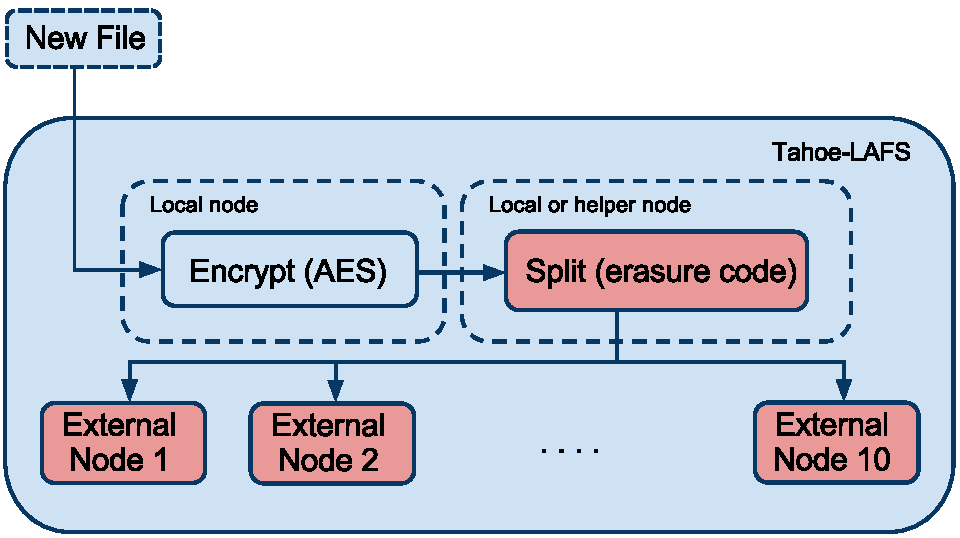
\includegraphics[width=0.9\columnwidth]{Tahoe-newfile.pdf}
    \caption{Tahoe-LAFS: Insertion of new file}
    \label{fig:tahoeinsertion}
\end{figure}

Tahoe was originally developed with funding from the former commercial web
backup service provider Allmydata, but is now a stand-alone Open
Source\footnote{GNU General Public License (GPL) version 2} project \cite{t_ars}.
It is written in the Python programming language with the Twisted framework, and
can run on Windows, Mac OSX, Linux, Solaris and more.



\subsection{Erasure coding}

The use of \emph{erasure coding} enables Tahoe to recover a file using only a
predefined subset of the parts distributed to the storage servers, i.e. the
other nodes in the grid. Erasure coding is a type of \ac{FEC} code, which
extends a message with $C$ characters into a longer message with $N$ symbols.
The original $C$ characters can then be recovered from a subset of the $N$
symbols.

The properties of erasure coding can be seen up on as those of recovery in RAID
systems.

% TODO: comparison with RAID?

\subsection{Use of secure hashes in Tahoe-LAFS}

% Describe hash trees in further detail?

\begin{figure}[h!]
    \centering
    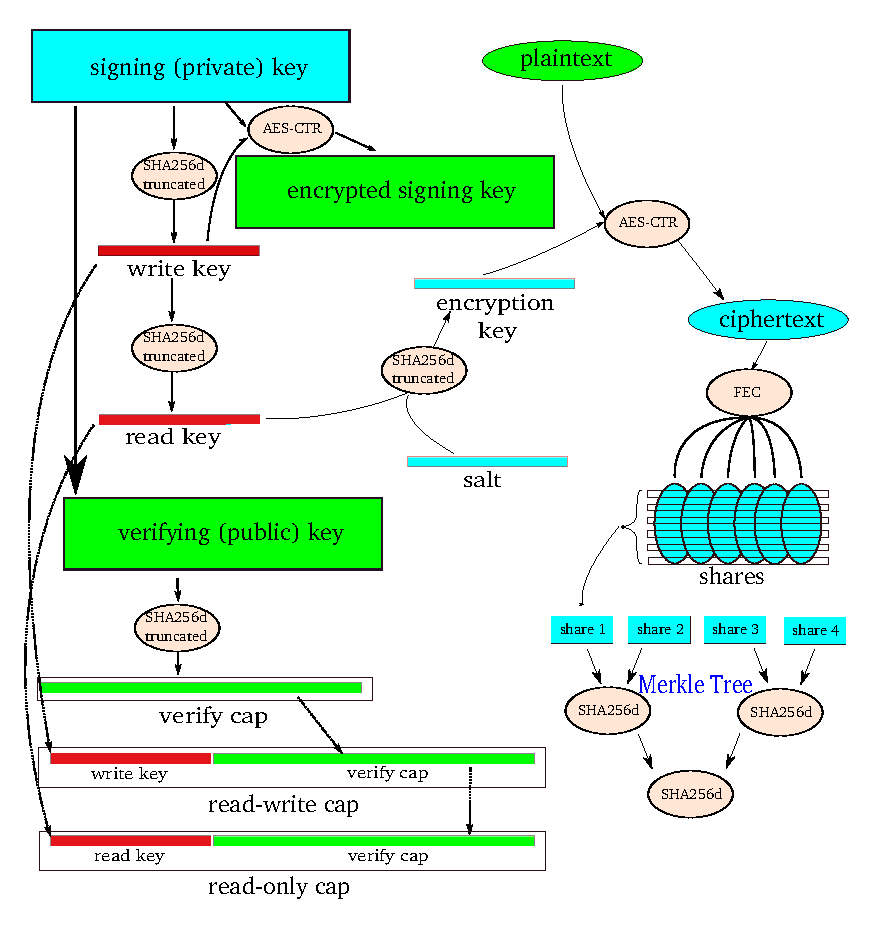
\includegraphics[width=0.9\columnwidth]{Tahoe-hashing.pdf}
    \caption{Tahoe-LAFS: Location of hashing}
    \label{fig:tahoehashing}
\end{figure}

As seen in figure \ref{fig:tahoehashing}, the usage of secure hashing is
extensive in Tahoe, and has to be considered as a key part of the functionality.


\section{Python bindings using Cython}
%What is it, how, why, alternatives?
% TODO: Hvorfor er nedenfornevnte i ASM eller C?
TAHOE-LAFS is written in python, but the SHA-3 candidate implementations found
in both the official NIST submissions and supercop are either in C or in
assembly. Therefore we need a way to make the implementations available in
Python. There a several ways to do this. Python itself includes a C-API,  
other options include SWIG, Cython and possible others.

\subsection{Python C-API}
The Python C-API is the official method of creating C-bindings for Python. The
procedure to do this includes writing entrypoints or wrappers for your C
functions in C. Then, through compiling you can acess your C-libraries and
functions through Python. The drawback with this approach, when faced with an
already existing C-library is that you have to actually write the
wrapper-functions or modify the C-library.

\subsection{Cython}
Cython tries to solve the problem of binding C-libraries and functions by the
use of Python instead of the use of C which the official API does. This is done
by only defining the entrypoints to the required C-functions and datatypes in a
Python/C/C++ hybrid syntax. Cython also allows creating new C/C++ functions,
available or not available to Python, in the same syntax. Cython works by
transforming the hybrid syntax into C/C++-code which utilises the official
Python C-API and compiling that. An expected tradeoff by using Cython is a
performance drop due to the extra layer of abstraction.


\chapter{Procedure}

TODO: We have to figure out a new title
Keywords: Python bindings in detail, unit tests, using it in Tahoe-LAFS

A bit more technical description of how we tested the candidates in Tahoe-LAFS

Limitations/assumptions

Optimized candidates.

Error sources.


\chapter{Results}

What is tested and what is not tested?

tables, graphs?


\chapter{Discussion}

What could have been done differently?

Compare results with general (supercop) results.

Optimized candidates.

\cite{s_nistround2}


\chapter{Conclusion}

A somewhat short conclusion summing up results and discussion

\section{Future work}

New SHA-3 capability in Tahoe-LAFS (GSOC ref) to get our code to trunk


% BibTeX bibliography lives in external file
\bibliographystyle{plain}
\bibliography{ref_sha3,ref_tahoe}

\appendix
\appendixpage
\addappheadtotoc

% Use ordinary \chapters from here on..

\end{document}
